\section{Mayer--Vietoris 序列}
\sourcepage{217}
若 $X=X_1\cup X_2$，在适当条件下，存在把 $X$ 的同调与 $X_1,X_2$ 的同调联系起来的正合列，称为这两个子空间的 \textbf{Mayer--Vietoris 序列}。单纯同调中，我们在 $X_1,X_2$ 是某个复形的子复形的多面体时构造过它。奇异同调需要类似的条件。

\entry{定义}{4.6.1}设 $X=X_1\cup X_2$，令 $\mathcal U=\{X_1,X_2\}$，记
\[
\mathcal S(X_1)+\mathcal S(X_2)=\mathcal S^{\mathcal U}(X).
\]
其 $p$ 维链群是 $S_p(X_1)+S_p(X_2)$；除非两个子空间不交，否则这不是直和。若包含映射
\[
\mathcal S(X_1)+\mathcal S(X_2)\longrightarrow\mathcal S(X)
\]
诱导同调同构，则称 $\{X_1,X_2\}$ 为\textbf{可切除对}（excisive couple）。

对于奇异同调，这一定义等价于第 3.5 节习题 3 中的定义，证明留作习题 2。由定理 4.4.8，若 $\Int X_1$ 与 $\Int X_2$ 覆盖 $X$，则它们构成可切除对。

\entry{定理}{4.6.2}设 $X=X_1\cup X_2$，$\{X_1,X_2\}$ 为可切除对，$A=X_1\cap X_2$。则有正合列
\[
\begin{split}
\cdots\longrightarrow H_p(A)\xrightarrow{\varphi_*}H_p(X_1)\oplus H_p(X_2)
\xrightarrow{\psi_*}H_p(X)\\
\xrightarrow{\partial_*}H_{p-1}(A)\longrightarrow\cdots,
\end{split}
\]
称为 $\{X_1,X_2\}$ 的 Mayer--Vietoris 序列。\translatornote{原书显示的序列漏印了 $H_p(X)$ 及其后的连接同态。}其中
\[
\varphi_*(a)=(i_*a,-j_*a),\qquad \psi_*(x_1,x_2)=k_*x_1+\ell_*x_2,
\]
而 $i:A\to X_1$、$j:A\to X_2$、$k:X_1\to X$、$\ell:X_2\to X$ 都是包含映射。若 $A\ne\varnothing$，约化同调也有类似序列。两种序列对连续映射诱导的同态都具有自然性。

\sourcepage{218}
\textbf{证明：}定义链复形的短正合列
\[
0\longrightarrow S_p(A)\xrightarrow{\varphi}S_p(X_1)\oplus S_p(X_2)
\xrightarrow{\psi}S_p(X_1)+S_p(X_2)\longrightarrow0,\tag{*}
\]
其中 $\varphi(c)=(i_\#c,-j_\#c)$，$\psi(c_1,c_2)=k_\#c_1+\ell_\#c_2$。映射 $\varphi$ 单射，$\psi$ 满射；其核由所有 $(c,-c)$ 组成，其中 $c$ 同时属于 $S_p(X_1)$、$S_p(X_2)$，即属于 $S_p(A)$。故序列正合。

之字形引理（引理 3.3.2）给出长正合列，而可切除性保证
\[
H_p(\mathcal S(X_1)+\mathcal S(X_2))\cong H_p(X).\tag{**}
\]
所以得到所需序列。若 $A\ne\varnothing$，同样论证可用于约化同调。

若 $f:(X,X_1,X_2)\to(Y,Y_1,Y_2)$ 连续，且两边均为可切除对，则 $f_\#$ 与包含映射可交换，因而与 $\varphi,\psi$ 可交换，给出短正合列间的同态，进而给出长正合列间的同态。同构 (**) 由包含映射诱导，也与 $f_*$ 可交换。这就证明了自然性。\hfill$\square$

下面给出 Mayer--Vietoris 序列的一个应用。回忆：若 $w_0*K$、$w_1*K$ 是两个锥，其多面体仅在 $|K|$ 相交，则并为 $K$ 的悬挂 $S(K)$（第 3.4 节）。映射
\[
\pi:|K|\times[-1,1]\to|S(K)|,\qquad
\pi(x,t)=\begin{cases}(1-t)x+tw_0,&t\ge0,\\(1+t)x-tw_1,&t\le0,\end{cases}
\]
是商映射，把 $|K|\times\{1\}$ 压缩为 $w_0$、把 $|K|\times\{-1\}$ 压缩为 $w_1$，在其余部分一一对应。\translatornote{原书第二行末项为 $+tw_1$；应为 $-tw_1$，使 $t=-1$ 时的像为 $w_1$。}证明与锥的相应结论类似（推论 2.8.8）。由此引出一般拓扑空间的悬挂。

\sourcepage{219}
\entry{定义}{4.6.3}空间 $X$ 的\textbf{悬挂}（suspension）是将 $X\times[-1,1]$ 中的 $X\times\{1\}$ 压缩为一点 $v$、将 $X\times\{-1\}$ 压缩为另一点 $w$ 所得的商空间，记为 $S(X)$。点 $v,w$ 称为\textbf{悬挂点}。

如同单纯同调的情形，可以用 Mayer--Vietoris 序列计算悬挂的同调。

\entry{定理}{4.6.4}对每个 $p$，存在同构 $\widetilde H_p(S(X))\to\widetilde H_{p-1}(X)$。

\textbf{证明：}令 $\pi:X\times[-1,1]\to S(X)$ 为商映射，$v,w$ 为两个悬挂点。取 $X_1=S(X)\setminus\{w\}$、$X_2=S(X)\setminus\{v\}$。它们都是开集，故为可切除对。下面证明两者无环，于是 Mayer--Vietoris 序列给出
\[
\widetilde H_p(S(X))\cong\widetilde H_{p-1}(X_1\cap X_2).
\]
还将证明 $X_1\cap X_2$ 同伦等价于 $X$，从而 $\widetilde H_{p-1}(X_1\cap X_2)\cong\widetilde H_{p-1}(X)$，即得结论。\translatornote{原书后一同构左端误印为 $\widetilde H_p(X_1\cap X_2)$；同伦等价诱导的是同维同调之间的同构。}

集合 $X\times(-1,1]$ 在 $X\times[-1,1]$ 中开，且关于 $\pi$ 饱和，故限制映射 $\pi':X\times(-1,1]\to X_1$ 是商映射。定义
\[
F:X\times(-1,1]\times I\to X\times(-1,1],\qquad
F(x,s,t)=(x,(1-t)s+t).
\]
它给出到 $X\times\{1\}$ 的形变收缩。复合 $\pi'\circ F$ 在 $\pi'\times i_I$ 的每个纤维上为常值，故诱导连续映射 $G:X_1\times I\to X_1$，使下图交换：
\[
\begin{array}{ccc}
X\times(-1,1]\times I&\xrightarrow{F}&X\times(-1,1]\\
\downarrow\scriptstyle\pi'\times i_I&&\downarrow\scriptstyle\pi'\\
X_1\times I&\xrightarrow{G}&X_1.
\end{array}
\]
\sourcepage{220}
这里由定理 2.8.2，$\pi'\times i_I$ 仍是商映射。映射 $G$ 给出 $X_1$ 到 $v$ 的形变收缩，所以 $X_1$ 无环。同理 $X_2$ 无环。

最后，限制映射 $\pi'':X\times(-1,1)\to X_1\cap X_2$ 是一一对应的商映射，故为同胚。而 $X\times\{0\}$ 是 $X\times(-1,1)$ 的形变收缩核，所以 $X$ 与 $X_1\cap X_2$ 同伦等价。\hfill$\square$

\entry{定义}{4.6.5}图 4.6.1 为\textbf{闭合的拓扑学家正弦曲线}（closed topologist's sine curve）。它是定义 4.2.11 中的正弦曲线与一条弧之并；该弧与原曲线仅在 $(0,-1)$、$(1,\sin1)$ 两点相交。习题 1 将用到它。
\begin{center}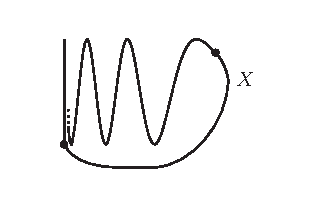
\includegraphics[width=.52\textwidth]{figures/4-6-1.pdf}\\图 4.6.1：闭合的拓扑学家正弦曲线\end{center}

\subsection*{习题}
\begin{enumerate}
\item 选取适当的 Mayer--Vietoris 序列，计算闭合的拓扑学家正弦曲线 $X$ 的奇异同调。
\item 证明：$\{X_1,X_2\}$ 为奇异同调中的可切除对，当且仅当包含映射 $(X_1,X_1\cap X_2)\to(X,X_2)$ 诱导奇异同调同构。〔提示：构造正合列
\[
0\to\mathcal S(X_2)\to\mathcal S(X_1)+\mathcal S(X_2)\to
\mathcal S(X_1)/\mathcal S(X_1\cap X_2)\to0,
\]
并把其导出的长正合列与 $\mathcal S(X,X_2)$ 的同调序列比较。〕
\item 证明 $n\ge1$ 时 $S^n$ 同胚于 $S(S^{n-1})$。利用这一事实计算 $S^n$ 的奇异同调。
\item 陈述并证明相对 Mayer--Vietoris 序列，其中中间的群为 $H_p(X_1,B_1)\oplus H_p(X_2,B_2)$，并假定 $\{X_1,X_2\}$、$\{B_1,B_2\}$ 均可切除。〔提示：把
\[
0\to\mathcal S(B_1\cap B_2)\to\mathcal S(B_1)\oplus\mathcal S(B_2)\to\mathcal S(B_1)+\mathcal S(B_2)\to0
\]
作为定理 4.6.2 证明中序列 (*) 的子序列，应用第 3.3 节习题 2 的蛇引理。〕
\item 设 $X=X_1\cup X_2$、$A=X_1\cap X_2$。假定 $X_1,X_2$ 在 $X$ 中闭，且 $A$ 是 $X_2$ 中某个开集 $U$ 的形变收缩核。证明 $X_1$ 是 $U\cup X_1$ 的形变收缩核，并证明 $\{X_1,X_2\}$ 可切除。
\item 设 $X_1$ 是闭上半圆，$X_2$ 是闭下半圆，$X$ 是平面中的完整单位圆。在这种情形，Mayer--Vietoris 序列给出什么结论？
\item 设 $X_1$ 是闭上半球面，$X_2$ 是闭下半球面，$X$ 是三维空间中的完整单位球面。在这种情形，Mayer--Vietoris 序列给出什么结论？
\end{enumerate}
